\chapter{相关理论与技术介绍}

\section{稀疏矩阵的压缩方式}

存储矩阵的一般方法是采用二维数组,其优点是可以随机地访问每一个元素,因而能够容易实现矩阵的各种运算。对于稀疏矩阵,它通常具有很大的维度,有时甚大到整个矩阵(零元素)占用了绝大部分内存采用二维数组的存储方法既浪费大量的存储单元来存放零元素,又要在运算中浪费大量的时间来进行零元素的无效运算。因此必须考虑对稀疏矩阵进行压缩存储(只存储非零元素)。

\subsection{COO Format}

最简单的稀疏矩阵的存储格式称为coordinate(COO) format,这个形式只保留哪些非0的值,分别使用三个数组:val, rolIdx, colIdx来对应存储数值、行号以及列号,这三个数组的大小都为矩阵非零元的个数NNZ。举例说明,
$$
\begin{pmatrix}
    \label{稀疏矩阵例子}
    1 & 0 & 0 & 0 & 0 \\
    2 & 4 & 0 & 6 & 0 \\
    3 & 0 & 5 & 0 & 0 \\
    4 & 7 & 0 & 8 & 9
\end{pmatrix}
$$

该矩阵在COO存储格式下,三个数组分别为:
\begin{lstlisting}[title=COO Format, frame=single]
val = {1, 2, 4, 6, 3, 5, 4, 7, 8, 9}
rolIdx = {0, 1, 1, 1, 2, 2, 3, 3, 3, 3}
colIdx = {0, 0, 1, 3, 0, 2, 0, 1, 3, 4}
\end{lstlisting}

\subsection{CSR Format}

CSR(Compressed Sparse Row)是一种按行压缩的矩阵存储形式。分别使用三个数组:val, rowPtr, colIdx来对应存储数值、行指针、以及列号。其中val和colIdx的数组大小为非零元的个数NNZ,而rowPtr数组的大小一般为m+1,其中 m 为矩阵行的个数。例如图\ref{CSR}。

\begin{figure}[htbp]
    \centering
    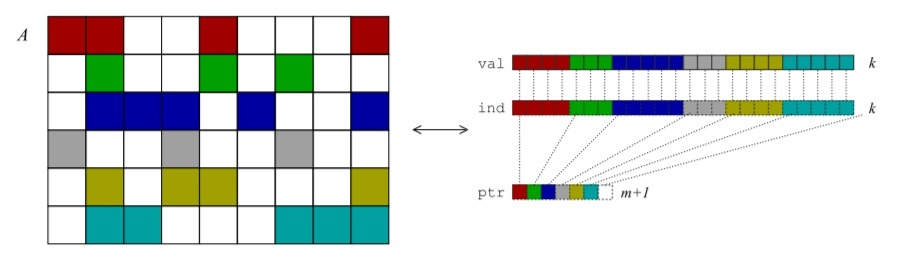
\includegraphics[width=0.7\textwidth]{CSR.png}
    \caption{CSR矩阵存储格式}
    \label{CSR}
\end{figure}

\subsection{CSC Format}

CSC(Compressed Sparse Column)与CSR相似,是一种按列压缩的矩阵存储格式。分别使用是那个数组:val, colPtr, rowIdx来对应存储数值、列指针、以及行号。其中val和rowIdx的数组大小为非零元的个数NNZ,而colPtr数组的大小一般为n+1,其中n为矩阵列的个数。例如图\ref{CSC}

\begin{figure}[htbp]
    \centering
    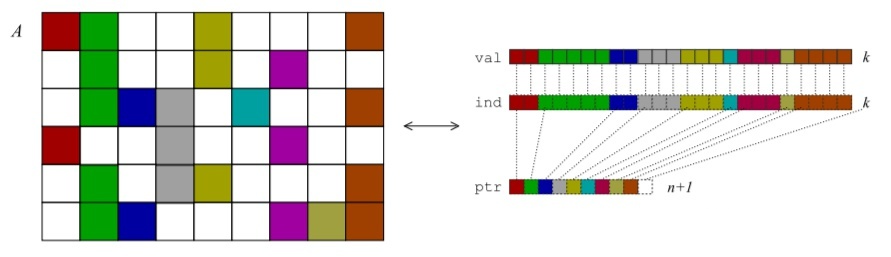
\includegraphics[width=0.7\textwidth]{CSC.png}
    \caption{CSC矩阵存储格式}
    \label{CSC}
\end{figure}

\section{SpTRSV串行算法}

\subsection{基于CSR格式的SpTRSV串行算法}

\subsection{基于CSC格式的SpTRSV串行算法}

\begin{algorithm}[htb]
    \caption{ Framework of ensemble learning for our system.}
    \label{alg:Framwork}
    \begin{algorithmic}[1]
      \State Extracting the set of reliable negative and/or positive samples $T_n$ from $U_n$ with help of $P_n$;
      \label{code:fram:extract}
      \State Training ensemble of classifiers $E$ on $T_n \cup P_n$, with help of data in former batches;
      \label{code:fram:trainbase}
      \State $E_n=E_{n-1}cup E$;
      \label{code:fram:add}
      \State Classifying samples in $U_n-T_n$ by $E_n$;
      \label{code:fram:classify}
      \State Deleting some weak classifiers in $E_n$ so as to keep the capacity of $E_n$;
      \label{code:fram:select} \\
      \Return $E_n$;
    \end{algorithmic}
  \end{algorithm}


\section{多核系统下的Cache一致性协议}

\section{ARM NEON指令}

\section{NUMA架构}

\section{本章小结}

\endinput